\documentclass[tikz,convert={density=300,size=300x300,outfile=\jobname.png}]{standalone}

\usetikzlibrary{automata,calc,trees,positioning,arrows,chains,shapes.geometric,%
decorations.pathreplacing,decorations.pathmorphing,shapes,%
matrix,shapes.symbols,plotmarks,decorations.markings,shadows}

\usepackage{subcaption}

\begin{document}

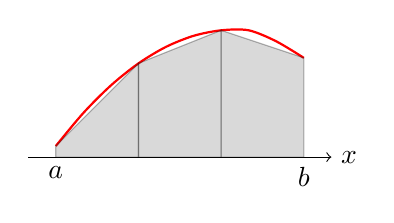
\begin{tikzpicture}[scale=0.7]
\draw[->] (-0.5,0)--(5,0) node[right] {$x$};
\node[below] at (0,0) {$a$};
\node[below] at (4.5,0) {$b$};
\draw [red, thick] plot [smooth] coordinates {
	(0.0, 0.20)
	(0.5, 0.80)
	(1.0, 1.30)
	(1.5, 1.70)
	(2.0, 2.00)
	(2.5, 2.20)
	(3.0, 2.30)
	(3.5, 2.30)
	(4.0, 2.10)
	(4.5, 1.80)
};
\draw [black, fill=gray, opacity=0.3] (0.0, 0.00) -- (0.0, 0.20) -- (1.5, 1.70) -- (1.5, 0.00) -- cycle;
\draw [black, fill=gray, opacity=0.3] (1.5, 0.00) -- (1.5, 1.70) -- (3.0, 2.30) -- (3.0, 0.00) -- cycle;
\draw [black, fill=gray, opacity=0.3] (3.0, 0.00) -- (3.0, 2.30) -- (4.5, 1.80) -- (4.5, 0.00) -- cycle;
\end{tikzpicture}
%\caption{Three Trapezoids}

\end{document}